%!TEX root = ../MasterThesis.tex

\section{\gls{RDF} vocabularies and Web Ontologies for \gls{E-commerce}}
\label{sec:choose_data_schema}

As a major objective of the \gls{E-commerce} fraud investigation system is to collect the various transactional information from online merchants, \gls{PSP}s and issuers, combine and link them together, as well as analyse the resulting data set from different view points to find abnormal activities, the information exchanged between the relevant participants either have to follow commonly available \gls{RDF} vocabularies, have to be based on a custom shared \gls{RDF} vocabulary that has been specifically designed for this system, or have to be mapped and linked against each other from different \gls{RDF} schema specifications.

\subsection{Reuse of common \gls{RDF} vocabularies}
\label{subsec:reuse_vocab_web}

One valid approach to come up with a data schema for the collaborative system is to take a look into commonly used \gls{RDF} vocabularies and Web ontologies, and try to figure out whether they can be used for describing the information that need to be exchanged between participants of the \gls{E-commerce} fraud investigation system. When consulting the Semantic Web community for commonly agreed upon and highly used \gls{RDF} schema specifications, one will come up with the following list (see Table~\ref{tab:used_vocab_rdf}):\@

\begin{table}[H]
\centering
\begin{tabular}{p{3cm}llp{4.5cm}}
\hline
\textbf{Name} & \textbf{Prefix} & \textbf{Describes} & \textbf{Namespace URI} \\
\hline
Dublin Core & dc: & Meta data & \url{http://purl.org/dc/terms/} \\
\hline
FOAF & foaf: & People & \url{http://xmlns.com/foaf/0.1/} \\
\hline
Geo & pos: & Positions & \url{http://www.w3.org/2003/01/geo/wgs84\_pos\#} \\
\hline
Geo Names & gn: & Locations & \url{http://www.geonames.org/ontology\#} \\
\hline
Good Relations & gr: & Products & \url{http://purl.org/goodrelations/v1\#} \\
\hline
RDF & rdf: & Core framework & \url{http://www.w3.org/1999/02/22-rdf-syntax-ns\#} \\
\hline
RDFS & rdfs: & RDF vocabularies & \url{http://www.w3.org/2000/01/rdf-schema\#} \\
\hline
Schema.org & schema: & Schema.org vocabularies & \url{http://schema.org/} \\
\hline
SKOS & skos: & Controlled vocabularies & \url{http://www.w3.org/2004/02/skos/core\#} \\
\hline
vCard & vcard: & Business Cards & \url{http://www.w3.org/2006/vcard/ns\#} \\
\hline
Web Ontology Language & owl: & Ontologies & \url{http://www.w3.org/2002/07/owl\#} \\
\hline
XML Schema Datatypes & xsd: & Data types & \url{http://www.w3.org/2001/XMLSchema\#} \\
\hline
\end{tabular}
\caption[Commonly used \gls{RDF} vocabularies on the Web]{Commonly used \gls{RDF} vocabularies on the Web \citep[pg. 41]{wood2014linked}}
\label{tab:used_vocab_rdf}
\end{table}

Based on these existing schema specifications describing a fictive consumer named ``Max Mustermann'' \gls{incl}\ his home address can be done by combining data utilizing the \gls{FOAF} and \gls{vCard} vocabularies into a \gls{RDF} data set such as described in Listing~\ref{lst:sample_customer_mustermann} and visualized as directed graph in Figure~\ref{fig:images_sample_customer}. The described resource is uniquely identified by the \gls{URI} \url{http://www.merchant1.com/customers/MaxMustermann}. Additionally, one can see that these vocabularies use expressive names for their entities and predicates, which make it easier to understand their intended meanings (e.g.\ ``foaf:givenname'', ``vcard:locality'', \ldots).  \@

\begin{listing}[H]
  \inputminted[linenos,
               numbersep=5pt,
               breaklines=true,
               frame=lines]{TURTLE}
               {./samples/sample_customer_mustermann.ttl}
  \caption{Personal related information about a fictive consumer in \gls{RDF}}
\label{lst:sample_customer_mustermann}
\end{listing}

\begin{figure}[H]
	\centering
		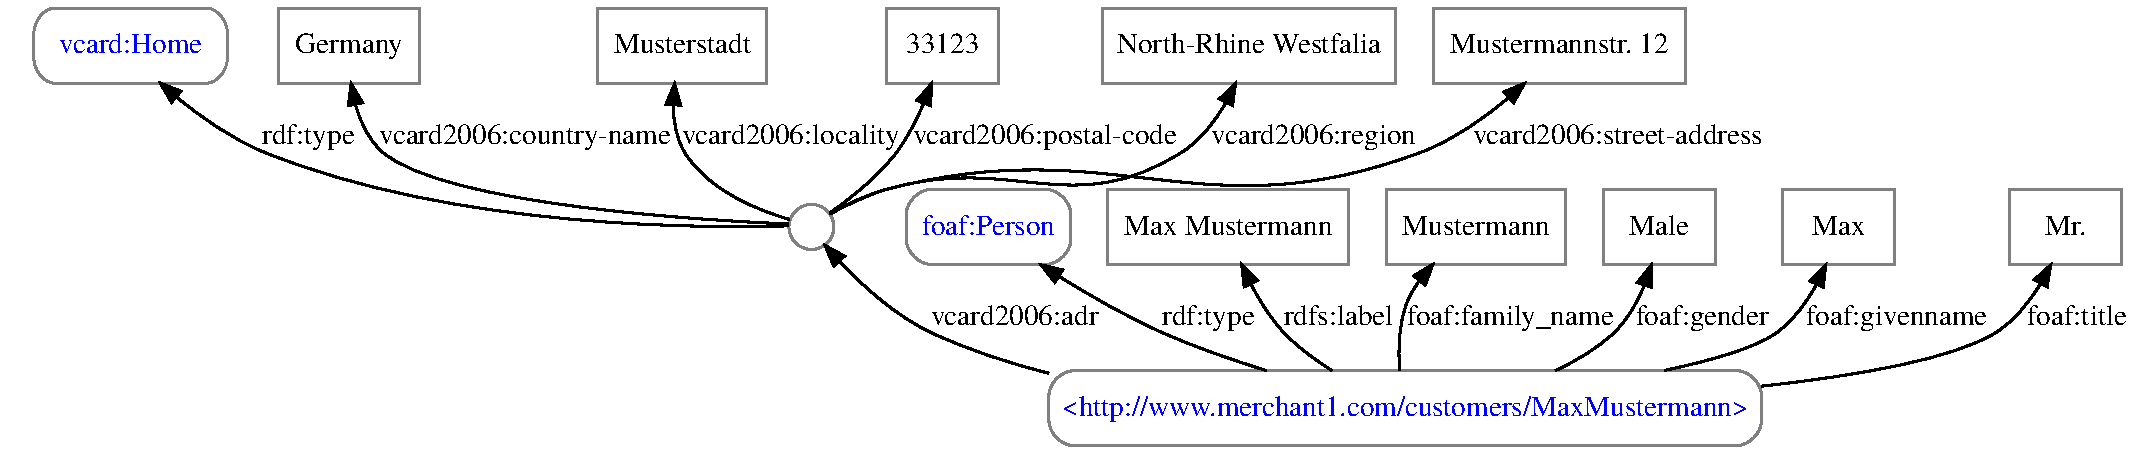
\includegraphics[width=\columnwidth]{images/sample_customer_mustermann.pdf}
	\caption{Graph representation of consumer information from Listing~\ref{lst:sample_customer_mustermann}}
\label{fig:images_sample_customer}
\end{figure}

However, being able to describe persons and their addresses is just a subset of the entities and relations found in the \gls{E-commerce} scenario. When looking back to the initial \gls{ER} model of an \gls{E-commerce} transaction as shown in Section~\ref{sec:data_model_transactions}, one can map the entities that are currently available in the \gls{E-commerce} scenario to the existing \gls{RDF} vocabularies such as follows (see Table~\ref{tab:map_tx_rdf_vocab}): \@

\begin{table}[H]
\centering
\begin{tabular}{p{5cm}l}
\hline
\textbf{Information} & \textbf{RDF vocabulary} \\
\hline
Consumer & FOAF \\
\hline
Credit Card Owner & FOAF \\
\hline
Billing Address & vCard \\
\hline
Shipping Address & vCard \\
\hline
Location Information & Geo Names \\
\hline
Merchant & GoodRelations \\
\hline
Items & GoodRelations \\
\hline
Item Categories & GoodRelations \\
\hline
Brands & GoodRelations \\
\hline
Payment Types & GoodRelations \\
\hline
\end{tabular}
\caption{Possible usage of \gls{RDF} vocabularies for \gls{E-commerce} transaction information}
\label{tab:map_tx_rdf_vocab}
\end{table}

As this table shows, there are some parts of the \gls{E-commerce} \gls{ER} model that can be expressed with existing \gls{RDF} vocabularies extensively such as personal related information via \gls{FOAF} and \gls{vCard}, whereas other parts can not be stated in-depth (e.g.\ credit card information), or are not specified at all (e.g.\ tracking of the delivery). Due to these circumstances one usually have to build an own \gls{RDF} vocabulary or Web ontology that fills in the missing pieces, and refers to the existing concepts whenever appropriate.\\

When trying to model the information of a credit card as displayed in Figure~\ref{fig:images_data_model} a possible result will be the \gls{RDFS} specification shown in Listing~\ref{lst:credit_card_vocab}. This definition of a credit card resource explicitly reuses entities from the \gls{FOAF} and GoodRelations ontologies by defining that: \@

\begin{itemize}
 \item the owner of a credit card has to be of type ``Person'' from the \gls{FOAF} ontology,
 \item the type of a credit card has to be an instance of the type ``PaymentMethodCreditCard'' from the GoodRelations ontology.
\end{itemize}

As most of the parts of the \gls{E-commerce} data model shown in Figure~\ref{fig:images_data_model} can not be expressed with the existing \gls{RDF} vocabularies directly, filling in the gaps would mean to come up with a large set of custom entities and relationships, which will limit the usage of the system as explained in Section~\ref{subsec:build_ontology_frauds}.

\begin{listing}[H]
 \inputminted[linenos,
              numbersep=5pt,
              breaklines=true,
              frame=lines]{TURTLE}
              {./samples/vocab_credit_card.ttl}
 \caption{A specification for a credit card in \gls{RDFS}}
\label{lst:credit_card_vocab}
\end{listing}

When analysing the list of existing and actively used \gls{RDF} vocabularies and Web ontologies in Table~\ref{tab:used_vocab_rdf}, one will also find the Schema.org initiative \citep{Schema.org}. This meta data vocabulary was initially designed by the leading search engines (e.g.\ Google, Microsoft and Yahoo!) to allow authors of Web sites to markup their \gls{HTML} documents in a way, so that they are better understood by these search engines. The Schema.org vocabulary is actively maintained by its community, includes new concepts with each release, and also offers an extension mechanism to implement additional vocabularies with terms that are not part of the core specifications \citep{SchemaExtensions} yet. In one of the past releases the maintainers also introduced all of the existing concepts of the GoodRelations ontology into the Schema.org vocabulary \citep{SchemaGoodRelation}. \\

As online merchants likely provide semantic meta data for their products and offerings in the vocabulary of Schema.org with the objective to improve their listings on search engine results (also known as \gls{SEO}) already, one can reuse parts of these information for the \gls{E-commerce} fraud investigation scenario. Additionally, the wide-ranging scope of aspects declared in the Schema.org vocabulary can make it a good fit for the collaborative system to support the investigation of \gls{E-commerce} frauds. When trying to map the initial \gls{ER} model from Section~\ref{sec:data_model_transactions} to the Schema.org core specifications, one will basically come up with a schema as displayed in Figure~\ref{fig:images_schema_org}. \@

\begin{figure}[H]
	\centering
		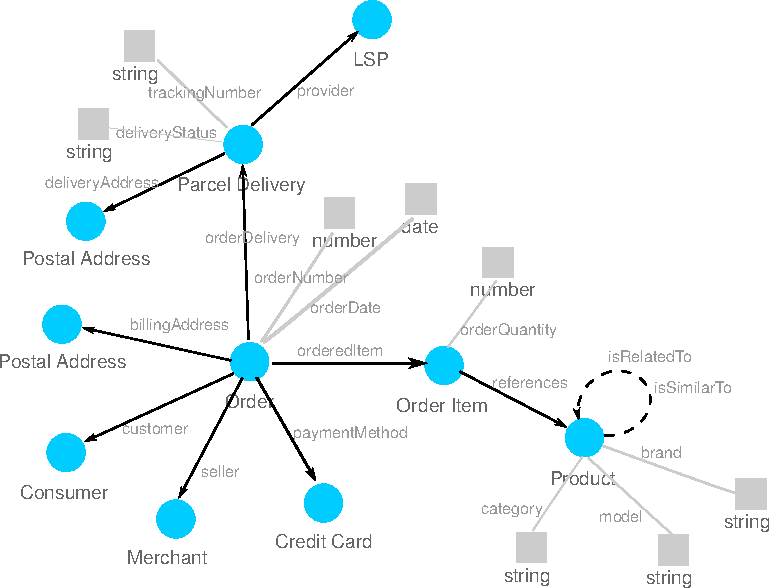
\includegraphics[width=0.8\columnwidth]{images/schema_org_mapping.pdf}
	\caption{Schema.org based mapping of an \gls{E-commerce} transaction}
\label{fig:images_schema_org}
\end{figure}

% subsection reuse_vocab_web (end)

\subsection{Creation of a custom \gls{RDF} vocabulary}
\label{subsec:build_ontology_frauds}

Another possible approach to harmonise information in the collaborative system is to define a completely new \gls{RDF} vocabulary or Web ontology for the proposed \gls{E-commerce} fraud investigation system, and share that with every possible stakeholder. This specification will have to define all the entities and relations known to the collaborative system and describe them in \gls{RDFS} format (see Section~\ref{sec:semantic_web}). \\

A major drawback of this approach is that new participants of the system will have to implement the conversion of their internal data structures to a \gls{RDF} data set that follows the predefined schema definition first, before even being able to join in. This will limit the general usage of the collaborative system, and will therefore not further considered in detail.

% subsection build ontology (end)

\subsection{Mapping of \gls{RDF} vocabularies}

Although it is possible to model an \gls{E-commerce} transaction solely with the Schema.org specifications as shown in Figure~\ref{fig:images_schema_org}, the collaborative system likely has to take care of the mapping of the transactional information coming from various sources to be able to combine them later. As the Semantic Web does not restrict how organizations structure and express their information, and due to the ``AAA slogan'' (see Section~\ref{sec:semantic_web}), there are likely different \gls{RDF} representations of an \gls{E-commerce} transaction in-use and have to be brought together. \\

The \gls{W3C} standards for the Semantic Web also include support for these mapping issues, because they will also come up when trying to combine semantic information available around the Web. The following axioms are available in the \gls{RDFS} and \gls{OWL} specifications explicitly for that purpose: \@

\begin{itemize}
	\item \textbf{rdfs:subClassOf:} a relation of type ``rdfs:subClassOf'' defines a specialization of a class, in which the child class inherits all the properties of the parent class,
  \item \textbf{rdfs:subProperyOf:} a relation of type ``rdfs:subPropertyOf'' defines a specialization of a property, in which the child property inherits all constraints of the parent property,
  \item \textbf{owl:equivalentClass:} a relation of type ``owl:equivalentClass'' specifies the equality of classes coming from different \gls{RDF} vocabularies or Web ontologies,
  \item \textbf{owl:equivalentProperty:} a relation of type ``owl:equivalentProperty'' specifies the equality of classes coming from different \gls{RDF} vocabularies or Web ontologies
\end{itemize}

If a merchant wants to state that a product related information, which is delivered as resource using the GoodRelations vocabulary, is equal to product information that can be found in the Schema.org specification, he or she can do so as follows (see Listing~\ref{lst:schema_mapping_gr_schema_org}): \@

\begin{listing}[H]
 \inputminted[linenos,
              numbersep=5pt,
              breaklines=true,
              frame=lines]{TURTLE}
              {./samples/mapping_gr_schema_org.ttl}
 \caption{Mapping product-related information from GoodRelations to Schema.org}
\label{lst:schema_mapping_gr_schema_org}
\end{listing}

These mapping statements from one \gls{RDF} vocabulary to another can be either created and injected into a \gls{RDF} data store by the party, who is going to merge information from different sources according to needs, or can also be part of the resource specification coming from an external source. In the former case the stakeholder, who is collecting and combining the information from various sources, has to maintain the additional triples to map information between each \gls{RDF} vocabulary used, and include them in the processing of the external statements within the combined \gls{RDF} data store. With an increased number of participants, who are using disjunct \gls{RDF} vocabularies, the effort and time to manage and create these mapping instructions on the collectors side will increase tremendously. Thus, the second approach is the preferred one. In that situation the \gls{RDF} description of an entity coming from an external source is already stating the mapping to one or more well-known \gls{RDF} vocabularies (e.g.\ the Schema.org specification mentioned above). This will reduce the effort and time to combine the information from different sources, and will only slightly increase the effort on the side of the external partner to prepare their internal information for external consumptions.

% subsection map ontology (end)

% sec data_schema (end)
